\documentclass[10pt]{article}
 
\usepackage[margin=1in]{geometry} 
\usepackage{amsmath,amsthm,amssymb, graphicx, multicol, array}
\usepackage{parskip}
 
\newcommand{\N}{\mathbb{N}}
\newcommand{\Z}{\mathbb{Z}}
 

\begin{document}
 
\title{Problem Set 2}
\author{Nicolas Moreno, Kushal Patel, Olivia Wilkinson \\
ECON: 880}
\maketitle

\section{Problem 1}

Assume that markets are complete. Since markets are complete and there are no additional externalities, the competitive equilibrium for this economy will be pareto efficient. We find the allocation]
with the planners problem and then back out the discount bond price. We solve

We solve 
\begin{align*}
    \max \sum_{t = 0}^{\infty} \beta^{t} \left[ \pi (e) \frac{c(e)^{1 - \alpha} - 1}{1 - \alpha} + (1 - \pi (e) ) \frac{c(u)^{1 - \alpha} - 1}{1 - \alpha}  \right] \\
    \text{ s.t } \pi (e) c(e) + (1 - \pi (e)) c(u) \leq \pi (e) y(e) + (1 - \pi (e)) y(u)
\end{align*}

First order conditions imply 
\[ \beta^{t} (1 - \alpha) c(e)^{- \alpha} =  \lambda_{t}\]
\[\beta^{t}  (1 - \alpha) c(u)^{- \alpha} =  \lambda_{t} \]
\[ \implies c(e) = c(u). \]

To find the invariant distribution , we solve 
\begin{equation*}
    \begin{bmatrix}
        \pi(e) \\
        \pi(u)
    \end{bmatrix} =
    \begin{bmatrix}
        0.97 & 0.50 \\
        0.03 & 0.50 \\
    \end{bmatrix}
    \begin{bmatrix}
        \pi(e) \\
        \pi(u)
    \end{bmatrix} 
\end{equation*}
along with the restriction $\pi(e) + \pi(e) = 1$ to obtain $\pi (e) \approx 0.9434$ and $ \pi (u) \approx 0.0566$. 

To find the price of the arrow security $q_t$ , we simply find the stochastic discount factor 
\[ \beta^{t} u'(c(s_{t})) q_{t} = \beta^{t+1} u'(c(s_{t+1})) \implies q_{t} = \beta = 0.9932, \]
where we used the first/second welfare theorem to note that allocations will be equalized across all states. 

\newpage
\section{Problem 2}

\subsection{Policy Function}

\begin{figure}[!h]
    \centering 
    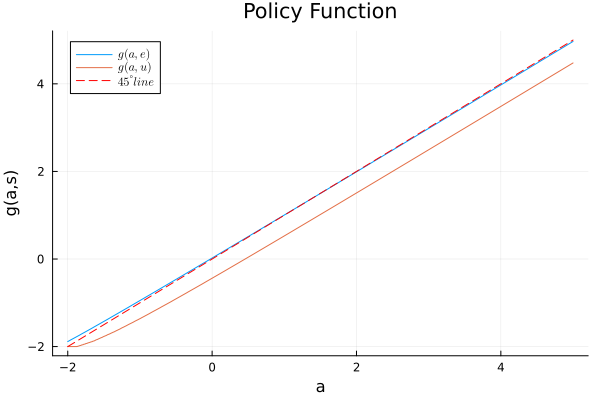
\includegraphics[width = 0.75\textwidth]{policy_function.png}
\end{figure}

The policy function plotted above shows that $\hat{\alpha} \approx 1.28$. 

\subsection{Invariant Distribution and Bond Price }
\begin{figure}[!h]
    \centering 
    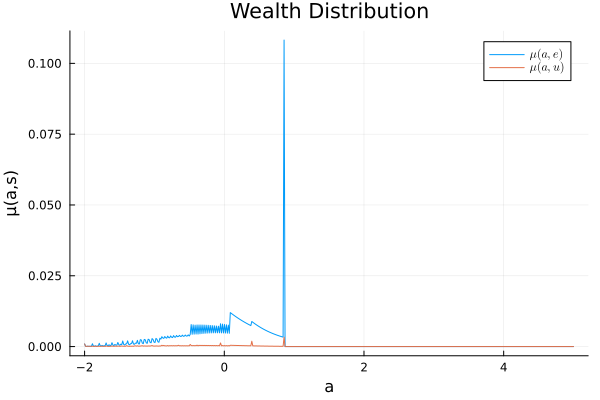
\includegraphics[width = 0.75\textwidth]{cross_sectional_distribution.png}
\end{figure}

The wealth distribution is plotted above. The discount bond price that clears the market is $ q \approx 0.9943$. 

\newpage
\subsection{Lorenz Curve and Gini Coefficient}
\begin{figure}[!h]
    \centering
    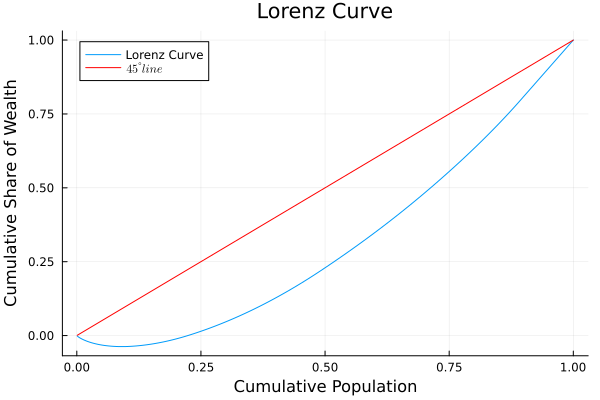
\includegraphics[width = 0.75\textwidth]{lorenz_curve.png}
\end{figure}

The lorenz curve is plotted above. The gini coefficient is $\approx 0.383$. 

\section{Problem 3}

\subsection{Welfare Analysis}

\begin{figure}[!h]
    \centering 
    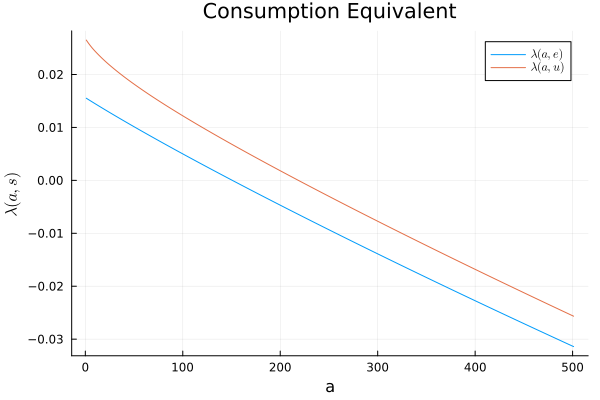
\includegraphics[width = 0.75\textwidth]{consumption_equiv.png}
\end{figure}

We plot the consumption equivalent above. Aggregate welfare with complete markets is -4.282945001004452
Aggregate welfare with incomplete markets is -4.45447969829158.
The aggregate welfare gain is 0.0011564081096912394.
The fractions of the population who would pay for complete markets is 0.5228655693555627.
\end{document}